\chapter{Klein Gordon Theory}

We have now developed the Hamiltonian formulation of \textbf{Classical Field Theory}, where the dynamical degrees of freedom are represented by the fields \(\phi_a(\mathbf{x}, t)\) and their conjugate momenta \(\pi_a(\mathbf{x}, t)\), which satisfy canonical Poisson brackets.
The next step is to promote this classical description to a \textbf{Quantum Field Theory (QFT)}, in which fields become operators acting on a Hilbert space, and classical observables become non-commuting operators.

\paragraph{From Classical Mechanics to Quantum Mechanics.}
The passage from classical to quantum mechanics provides a useful template.
In \textbf{Classical Mechanics (CM)}, a system with \(n\) degrees of freedom is described by canonical variables \((q_i, p_i)\), whose dynamics is determined by Hamilton’s equations:
\[
    \dot{q}_i = \frac{\partial H}{\partial p_i}, \qquad
    \dot{p}_i = -\frac{\partial H}{\partial q_i},
\]
and whose Poisson brackets encode the symplectic structure:
\[
    \{ q_i, p_j \} = \delta_{ij}.
\]

In \textbf{Quantum Mechanics (QM)}, the canonical variables are promoted to Hermitian operators \((\hat{q}_i, \hat{p}_i)\) on a Hilbert space, with the replacement
\[
    \{ \cdot, \cdot \} \;\longrightarrow\; \frac{1}{i\hbar} [\cdot, \cdot],
\]
leading to the canonical commutation relations
\[
    [\hat{q}_i, \hat{p}_j] = i\hbar \, \delta_{ij}.
\]
Observables evolve according to the Heisenberg equation
\[
    i\hbar \frac{d\hat{A}}{dt} = [\hat{A}, \hat{H}].
\]

\paragraph{From Classical Field Theory to Quantum Field Theory.}
The same canonical quantization idea extends to continuous systems.
Here we adopt the \textbf{Schr\"odinger picture}, in which operators are constant in time while states evolve.

In Classical Field Theory, the generalized coordinates are fields \(\phi_a(\mathbf{x}, t)\), and the conjugate momenta are
\[
    \pi_a(\mathbf{x}, t) = \frac{\partial \mathcal{L}}{\partial \dot{\phi}_a(\mathbf{x}, t)},
\]
with canonical Poisson brackets
\[
    \{ \phi_a(\mathbf{x}, t), \pi_b(\mathbf{y}, t) \} = \delta_{ab} \, \delta^{(3)}(\mathbf{x} - \mathbf{y}).
\]
The Hamiltonian functional
\[
    H[\phi, \pi] = \int d^3x \, \mathcal{H}(\phi_a, \pi_a, \nabla\phi_a)
\]
generates the time evolution of the fields.

In \textbf{Quantum Field Theory}, the fields become operators on a Hilbert (or Fock) space:
\[
    \phi_a(\mathbf{x}, t) \;\longrightarrow\; \hat{\phi}_a(\mathbf{x}),
    \qquad
    \pi_a(\mathbf{x}, t) \;\longrightarrow\; \hat{\pi}_a(\mathbf{x}),
\]
and the Poisson brackets are replaced by equal-time commutation relations:
\[
    [\hat{\phi}_a(\mathbf{x}), \hat{\pi}_b(\mathbf{y})] = i\hbar \, \delta_{ab}\, \delta^{(3)}(\mathbf{x}-\mathbf{y}), \qquad
[\hat{\phi}_a(\mathbf{x}), \hat{\phi}_b(\mathbf{y})] = [\hat{\pi}_a(\mathbf{x}), \hat{\pi}_b(\mathbf{y})] = 0,
\]
defining operators acting on the Fock space which can be written in terms of \textit{ladder operators} (annihilation and creation operators) acting on the vacuum.

In the Schr\"odinger picture, the states \(\ket{\psi(t)}\) evolve according to the Schr\"odinger equation:
\[
    i\hbar \frac{d}{dt} \ket{\psi(t)} = \hat{H} \ket{\psi(t)},
\]
where the wave functional \(\psi[\phi, t]\) encodes the probability amplitude for the field configuration \(\phi(\mathbf{x})\) at time \(t\).

Solving the theory requires diagonalizing the Hamiltonian \(\hat{H}\), which is generally difficult due to the infinite number of degrees of freedom and possible discrete or continuous field labels.
An important exception is \textbf{free theories} with quadratic Lagrangians, where the equations of motion are linear and can be solved exactly (e.g., the continuum limit of an elastic string).

Thus, canonical quantization provides a direct bridge from the Hamiltonian structure of classical fields to the operator formalism of quantum theory, where particles naturally arise as quantized excitations of the underlying fields.

\section{The Klein-Gordon Field as a Set of Harmonic Oscillators}

The simplest relativistic free field theory is the Klein-Gordon theory for a real scalar field \(\psi(\mathbf{x},t)\). Its \textbf{Lagrangian density} is
\begin{equation}
    \mathcal{L} = \frac{1}{2} \partial_\mu \psi \, \partial^{\mu} \psi - \frac{1}{2} m^2 \psi^2,
    \label{eq:KG_Lagrangian}
\end{equation}
and the corresponding \textbf{classical equations of motion}, obtained via the Euler-Lagrange procedure, read
\begin{equation}
    (\Box + m^2)\psi(x) = 0, \qquad \Box = \partial_\mu \partial^{\mu}.
    \label{eq:KG_motion_equations}
\end{equation}

\begin{remark}
    Although the Klein-Gordon equation appears as a single field equation in coordinate space, it is effectively a \emph{coupled system} of infinitely many degrees of freedom: the Laplacian term \(-\nabla^2 \psi\) couples the field at different spatial points.
    By performing a spatial Fourier transform, one can \emph{decouple} the system, obtaining independent harmonic oscillators for each momentum mode \(\mathbf{k}\).
    In momentum space, each mode evolves independently and can be quantized separately.
\end{remark}

We perform a spatial Fourier transform of the field:
\[
    \psi(t,\mathbf{x}) = \int \frac{\mathrm{d}^3 \mathbf{p}}{(2\pi)^3} \, e^{i \mathbf{p}\cdot \mathbf{x}} \tilde{\psi}(t,\mathbf{p}).
\]
The Klein-Gordon equation in momentum space becomes
\[
    \left[\frac{\partial^2}{\partial t^2} + \omega_{\mathbf{p}}^2 \right] \tilde{\psi}(t, \mathbf{p}) = 0,
    \qquad \omega_{\mathbf{p}} = \sqrt{|\mathbf{p}|^2 + m^2}.
\]
This shows explicitly that the system reduces to an infinite set of \emph{decoupled harmonic oscillators}, one for each momentum mode \(\mathbf{p}\).

\subsection{Canonical Quantization in Momentum Space}

Following the analogy with the quantum harmonic oscillator in quantum mechanics, each momentum mode can be quantized independently.
Recall that for a single harmonic oscillator with mass \(m=1\) and frequency \(\omega\), the canonical operators satisfy
\[
    \hat{q} = \frac{1}{\sqrt{2\omega}} (\hat{a} + \hat{a}^{\dagger}), \qquad
    \hat{p} = -i \sqrt{\frac{\omega}{2}} (\hat{a} - \hat{a}^{\dagger}),
\]
where \(\hat{a}, \hat{a}^\dagger\) are the annihilation and creation operators, obeying \([\,\hat{a}, \hat{a}^\dagger\,] = 1\).

We can generalize this construction to the field operators. A general solution to the Klein-Gordon equation (satisfying reality of the field) can be written as
\[
    \hat{\psi}(\mathbf{x}) = \int \frac{\mathrm{d}^3 \mathbf{p}}{(2\pi)^3} \frac{1}{\sqrt{2 \omega_{\mathbf{p}}}} \Big[ \hat{a}_{\mathbf{p}} e^{i \mathbf{p}\cdot \mathbf{x}} + \hat{a}_{\mathbf{p}}^\dagger e^{-i \mathbf{p}\cdot \mathbf{x}} \Big],
\]
with conjugate momentum operator
\[
    \hat{\pi}(\mathbf{x}) = \int \frac{\mathrm{d}^3 \mathbf{p}}{(2\pi)^3} \, (-i) \sqrt{\frac{\omega_{\mathbf{p}}}{2}} \Big[ \hat{a}_{\mathbf{p}} e^{i \mathbf{p}\cdot \mathbf{x}} - \hat{a}_{\mathbf{p}}^\dagger e^{-i \mathbf{p}\cdot \mathbf{x}} \Big],
\]
where the ladder operators acts on the Fock space creating and destroying particles of momentum \(\mathbf{p}\) (or \(\mathbf{q}\)).
Furthermore, they satisfy the canonical commutation relations:
\[
    [\,\hat{a}_{\mathbf{p}}, \hat{a}_{\mathbf{q}}\,] = [\,\hat{a}_{\mathbf{p}}^\dagger, \hat{a}_{\mathbf{q}}^\dagger\,] = 0, \qquad
    [\,\hat{a}_{\mathbf{p}}, \hat{a}_{\mathbf{q}}^\dagger\,] = (2\pi)^3 \delta^3(\mathbf{p} - \mathbf{q}).
\]

Our solutions now have to respect similar canonical commutation relations. In fact we know that:
\[
    \begin{aligned}
        [\,\hat{\psi}(\mathbf{x}),\hat{\pi}(\mathbf{y})\,]  & = i \delta^3 (\mathbf{x} - \mathbf{y}), \text{ while}    \\
        [\,\hat{\psi}(\mathbf{x}),\hat{\psi}(\mathbf{y})\,] & = [\,\hat{\pi}(\mathbf{x}),\hat{\pi}(\mathbf{y})\,] = 0.
    \end{aligned}
\]
Let us show this results:
\[
    \begin{aligned}
        [\,\hat{\psi}(\mathbf{x}),\hat{\pi}(\mathbf{y})\,] & = \int \frac{\mathrm{d}^3 \mathbf{p}\mathrm{d}^3 \mathbf{q}}{(2\pi)^6} \, \frac{(-i)}{2} \sqrt{\frac{\omega_{\mathbf{q}}}{\omega_{\mathbf{p}}}} \left[ \,\hat{a}_{\mathbf{p}} e^{i \mathbf{p}\cdot \mathbf{x}} + \hat{a}_{\mathbf{p}}^\dagger e^{-i \mathbf{p}\cdot \mathbf{x}}\, , \,\hat{a}_{\mathbf{q}} e^{i \mathbf{q}\cdot \mathbf{y}} - \hat{a}_{\mathbf{q}}^\dagger e^{-i \mathbf{q}\cdot \mathbf{y}} \, \right]  \\
                                                           & = \int \frac{\mathrm{d}^3 \mathbf{p}\mathrm{d}^3 \mathbf{q}}{(2\pi)^6} \, \frac{(-i)}{2} \sqrt{\frac{\omega_{\mathbf{q}}}{\omega_{\mathbf{p}}}} \left[ - [\,\hat{a}_{\mathbf{p}}, \hat{a}_{\mathbf{q}}^\dagger\,] e^{i (\mathbf{p} \cdot \mathbf{x} - \mathbf{q} \cdot \mathbf{y})} + [\,\hat{a}^\dagger_{\mathbf{p}}, \hat{a}_{\mathbf{q}}\,] e^{-i (\mathbf{p} \cdot \mathbf{x} - \mathbf{q} \cdot \mathbf{y})}\right] \\
                                                           & = \int \frac{\mathrm{d}^3 \mathbf{p}\mathrm{d}^3 \mathbf{q}}{(2\pi)^6} \, \frac{(-i)}{2} \sqrt{\frac{\omega_{\mathbf{q}}}{\omega_{\mathbf{p}}}} (2\pi)^3\left[ - \delta^3(\mathbf{p} - \mathbf{q})e^{i (\mathbf{p} \cdot \mathbf{x} - \mathbf{q} \cdot \mathbf{y})} + (- \delta^3(\mathbf{q} - \mathbf{p}))e^{-i (\mathbf{p} \cdot \mathbf{x} - \mathbf{q} \cdot \mathbf{y})}\right]                                     \\
                                                           & = \int \frac{\mathrm{d}^3 \mathbf{p}}{(2\pi)^3} \, \frac{i}{2} \sqrt{\frac{\omega_{\mathbf{q}}}{\omega_{\mathbf{p}}}} \left[ \delta^3(\mathbf{p} - \mathbf{q})\left(e^{i (\mathbf{p} \cdot \mathbf{x} - \mathbf{q} \cdot \mathbf{y})} + e^{-i (\mathbf{p} \cdot \mathbf{x} - \mathbf{q} \cdot \mathbf{y})}\right) \right]                                                                                                \\
                                                           & = \frac{i}{2} \int \frac{\mathrm{d}^3 \mathbf{p}}{(2\pi)^3} \, \sqrt{\frac{\omega_{\mathbf{p}}}{\omega_{\mathbf{p}}}} \left( e^{i \mathbf{p} \cdot (\mathbf{x} - \mathbf{y})} + e^{-i \mathbf{p} \cdot (\mathbf{x} - \mathbf{y})}\right)                                                                                                                                                                                 \\
                                                           & =  \frac{i}{2} \int \frac{\mathrm{d}^3 \mathbf{p}}{(2\pi)^3} \,  e^{i \mathbf{p} \cdot (\mathbf{x} - \mathbf{y})} + \frac{i}{2} \int \frac{\mathrm{d}^3 \mathbf{p}}{(2\pi)^3} \, e^{i \mathbf{p} \cdot (\mathbf{y} - \mathbf{x})}                                                                                                                                                                                        \\
                                                           & = \frac{i}{2} \delta^3(\mathbf{x} - \mathbf{y}) + \frac{i}{2} \delta^3(\mathbf{y} - \mathbf{x}) = i \delta^3(\mathbf{x} - \mathbf{y}),
    \end{aligned}
\]
where in the first step we simplified the null commutators of the ladder operators, while in the last steps we recognized the integral representation of the Dirac delta function
\[
    \delta^3(\mathbf{x}) = \int \frac{\mathrm{d}^3 \mathbf{p}}{(2\pi)^3} \,  e^{\pm i \mathbf{p}\cdot\mathbf{x}}
\]
which is by definition the Fourier transform of a constant and it respects the property
\[
    \delta(\alpha \mathbf{x}) = \frac{\delta(\mathbf{x})}{\vert \alpha \vert}, \quad \to \quad \delta(-\mathbf{x}) = \delta(\mathbf{x}).
\]
For the other commutators we do not have to report the full computation, we need only to pay attention to the change in the signs with respect to the previous computation:
\[
    \begin{aligned}
        [\,\hat{\psi}(\mathbf{x}),\hat{\psi}(\mathbf{y})\,] & = \int \frac{\mathrm{d}^3 \mathbf{p}\mathrm{d}^3 \mathbf{q}}{(2\pi)^6} \, \frac{1}{2\sqrt{\omega_{\mathbf{q}}\omega_{\mathbf{p}}}} \left[ \,\hat{a}_{\mathbf{p}} e^{i \mathbf{p}\cdot \mathbf{x}} + \hat{a}_{\mathbf{p}}^\dagger e^{-i \mathbf{p}\cdot \mathbf{x}}\, , \,\hat{a}_{\mathbf{q}} e^{i \mathbf{q}\cdot \mathbf{y}} + \hat{a}_{\mathbf{q}}^\dagger e^{-i \mathbf{q}\cdot \mathbf{y}} \, \right] \\
                                                            & = \int \frac{\mathrm{d}^3 \mathbf{p}\mathrm{d}^3 \mathbf{q}}{(2\pi)^6} \, \frac{1}{2\sqrt{\omega_{\mathbf{q}}\omega_{\mathbf{p}}}} \left[ [\,\hat{a}_{\mathbf{p}}, \hat{a}_{\mathbf{q}}^\dagger\,] e^{i (\mathbf{p} \cdot \mathbf{x} - \mathbf{q} \cdot \mathbf{y})} + [\,\hat{a}^\dagger_{\mathbf{p}}, \hat{a}_{\mathbf{q}}\,] e^{-i (\mathbf{p} \cdot \mathbf{x} - \mathbf{q} \cdot \mathbf{y})}\right]  \\
                                                            & = \frac{1}{2} \int \frac{\mathrm{d}^3 \mathbf{p}}{(2\pi)^3} \, \frac{1}{\omega_{\mathbf{p}}} \left( e^{i \mathbf{p} \cdot (\mathbf{x} - \mathbf{y})} - e^{-i \mathbf{p} \cdot (\mathbf{x} - \mathbf{y})}\right) \propto \delta^3(\mathbf{x} - \mathbf{y}) - \delta^3(\mathbf{y} - \mathbf{x}) = 0;
    \end{aligned}
\]
similarly:
\[
    \begin{aligned}
        [\,\hat{\pi}(\mathbf{x}),\hat{\pi}(\mathbf{y})\,] & = \int \frac{\mathrm{d}^3 \mathbf{p}\mathrm{d}^3 \mathbf{q}}{(2\pi)^6} \, \frac{(-i)^2}{2}\sqrt{\omega_{\mathbf{q}}\omega_{\mathbf{p}}} \left[ \,\hat{a}_{\mathbf{p}} e^{i \mathbf{p}\cdot \mathbf{x}} - \hat{a}_{\mathbf{p}}^\dagger e^{-i \mathbf{p}\cdot \mathbf{x}}\, , \,\hat{a}_{\mathbf{q}} e^{i \mathbf{q}\cdot \mathbf{y}} - \hat{a}_{\mathbf{q}}^\dagger e^{-i \mathbf{q}\cdot \mathbf{y}} \, \right] \\
                                                          & = \int \frac{\mathrm{d}^3 \mathbf{p}\mathrm{d}^3 \mathbf{q}}{(2\pi)^6} \, \frac{(-1)}{2}\sqrt{\omega_{\mathbf{q}}\omega_{\mathbf{p}}} \left[ - [\,\hat{a}_{\mathbf{p}}, \hat{a}_{\mathbf{q}}^\dagger\,] e^{i (\mathbf{p} \cdot \mathbf{x} - \mathbf{q} \cdot \mathbf{y})} - [\,\hat{a}^\dagger_{\mathbf{p}}, \hat{a}_{\mathbf{q}}\,] e^{-i (\mathbf{p} \cdot \mathbf{x} - \mathbf{q} \cdot \mathbf{y})}\right]  \\
                                                          & = \frac{1}{2} \int \frac{\mathrm{d}^3 \mathbf{p}}{(2\pi)^3} \, \omega_{\mathbf{p}} \left( e^{i \mathbf{p} \cdot (\mathbf{x} - \mathbf{y})} - e^{-i \mathbf{p} \cdot (\mathbf{x} - \mathbf{y})}\right) \propto \delta^3(\mathbf{x} - \mathbf{y}) - \delta^3(\mathbf{y} - \mathbf{x}) = 0.
    \end{aligned}
\]

\subsection{Hamiltonian and Ladder Operators}

Let us examine the classical Klein-Gordon Hamiltonian:
\[
    H = \int \mathrm{d}^3 \mathbf{x}\, T^{00} = \int \mathrm{d}^{3}\mathbf{x}\, (\pi \dot{\psi} - \mathcal{L}),
\]
where we have used the \textit{Legendre} transform to express the Hamiltonian density $T^{00}$. Here, \(\pi\) is the conjugate momentum of the field, and we recall that the Lagrangian density \(\mathcal{L}\) for a real scalar field is:
\[
    \mathcal{L} = \frac{1}{2} \partial_\mu \psi \partial^\mu \psi -\frac{1}{2} m^2 \psi^2 = \frac{1}{2}\left( \dot{\psi}^2 - \vert \nabla \psi \vert^2 - m^2 \psi^2 \right).
\]
Proceeding with the computation, and utilizing the relationship \(\pi = \frac{\partial \mathcal{L}}{\partial \dot{\psi}} = \dot{\psi}\), we simplify the total Hamiltonian to:
\[
    \begin{aligned}
        H & = \int \mathrm{d}^3 \mathbf{x}\, \left( \pi^2 -\frac{1}{2}\pi^2 + \frac{1}{2}\vert \nabla \psi \vert^2 + \frac{m^2}{2} \psi^2 \right) \\
          & = \frac{1}{2} \int \mathrm{d}^3 \mathbf{x}\, \left( \pi^2 + \vert \nabla \psi \vert^2 + m^2 \psi^2 \right) .
    \end{aligned}
\]

Now, to quantize the system, we promote the classical fields \(\psi\) and \(\pi\) to operators acting on a Fock Space within the \textbf{Schrödinger picture} (where operators have no explicit time dependence). We quantize via Fourier transform, which introduces the convenient definitions of the ladder operators:
\[
    \hat{\psi} (x) = \int \frac{\mathrm{d}^3 \mathbf{p}}{(2\pi)^3}\,\frac{1}{\sqrt{2\omega_{\mathbf{p}}}} \left[ \hat{a}_{\mathbf{p}}e^{i \mathbf{p} \cdot \mathbf{x}} + \hat{a}^{\dagger}_{\mathbf{p}} e^{-i \mathbf{p} \cdot \mathbf{x}} \right],
\]
where \(\omega_{\mathbf{p}} = \sqrt{\vert \mathbf{p} \vert^2 + m^2}\), and
\[
    \hat{\pi} (x) = \int \frac{\mathrm{d}^3 \mathbf{p}}{(2\pi)^3}\,(-i)\sqrt{\frac{\omega_{\mathbf{p}}}{2}} \left[ \hat{a}_{\mathbf{p}}e^{i \mathbf{p} \cdot \mathbf{x}} - \hat{a}^{\dagger}_{\mathbf{p}} e^{-i \mathbf{p} \cdot \mathbf{x}} \right].
\]
The promoted Hamiltonian operator now takes the form:
\[
    \hat{H} = \frac{1}{2} \int \mathrm{d}^3 \mathbf{x} \left( \hat{\pi}^2 + \vert \nabla \hat{\psi} \vert^2 + m^2 \hat{\psi}^2 \right).
\]
We compute the integrands of the individual squared terms (implicitly involving a double momentum integral $\int d^3\mathbf{p} d^3\mathbf{q}$):
\[
    \begin{aligned}
        \hat{\pi}^2                     & = - \frac{\sqrt{\omega_{\mathbf{p}} \omega_{\mathbf{q}}}}{2}\left[ \hat{a}_{\mathbf{p}}e^{i \mathbf{p} \cdot \mathbf{x}} - \hat{a}^{\dagger}_{\mathbf{p}} e^{-i \mathbf{p} \cdot \mathbf{x}} \right]\left[ \hat{a}_{\mathbf{q}}e^{i \mathbf{q} \cdot \mathbf{x}} - \hat{a}^{\dagger}_{\mathbf{q}} e^{-i \mathbf{q} \cdot \mathbf{x}} \right],                         \\
        \vert \nabla \hat{\psi} \vert^2 & = \frac{1}{2 \sqrt{\omega_{\mathbf{p}} \omega_{\mathbf{q}}}} i \mathbf{p}\left[ \hat{a}_{\mathbf{p}}e^{i \mathbf{p} \cdot \mathbf{x}} - \hat{a}^{\dagger}_{\mathbf{p}} e^{-i \mathbf{p} \cdot \mathbf{x}} \right]i\mathbf{q}\left[ \hat{a}_{\mathbf{q}}e^{i \mathbf{q} \cdot \mathbf{x}} - \hat{a}^{\dagger}_{\mathbf{q}} e^{-i \mathbf{q} \cdot \mathbf{x}} \right], \\
        m^2 \hat{\psi}^2                & = \frac{m^2}{2 \sqrt{\omega_{\mathbf{p}} \omega_{\mathbf{q}}}}\left[ \hat{a}_{\mathbf{p}}e^{i \mathbf{p} \cdot \mathbf{x}} + \hat{a}^{\dagger}_{\mathbf{p}} e^{-i \mathbf{p} \cdot \mathbf{x}} \right]\left[ \hat{a}_{\mathbf{q}}e^{i \mathbf{q} \cdot \mathbf{x}} + \hat{a}^{\dagger}_{\mathbf{q}} e^{-i \mathbf{q} \cdot \mathbf{x}} \right] .
    \end{aligned}
\]
By substituting these expressions into the Hamiltonian, performing the spatial integration, and simplifying (full computation detailed in Appendix \ref{app:computations}), we arrive at the final form:
\[
    \hat{H} = \frac{1}{2} \int \frac{\mathrm{d}^3 \mathbf{p}}{(2\pi)^3} \, \omega_{\mathbf{p}}\left( \hat{a}_{\mathbf{p}} \hat{a}^{\dagger}_{\mathbf{p}} + \hat{a}^{\dagger}_{\mathbf{p}} \hat{a}_{\mathbf{p}} \right),
\]
which depends solely on the ladder operators. Manipulating this expression slightly by recalling the canonical commutation relation for the operators:
\[
    [\,\hat{a}_{\mathbf{p}}, \hat{a}_{\mathbf{q}}^\dagger\,] = (2\pi)^3 \delta^3(\mathbf{p} - \mathbf{q}),
\]
we find that the Hamiltonian contains a fundamental divergence:
\[
    \hat{H} = \frac{1}{2} \int \frac{\mathrm{d}^3 \mathbf{p}}{(2\pi)^3} \, \omega_{\mathbf{p}}\left( 2 \hat{a}^{\dagger}_{\mathbf{p}} \hat{a}_{\mathbf{p}} + [\,\hat{a}_{\mathbf{p}}, \hat{a}_{\mathbf{p}}^\dagger\,] \right) = \int \frac{\mathrm{d}^3 \mathbf{p}}{(2\pi)^3} \, \omega_{\mathbf{p}} \hat{a}^{\dagger}_{\mathbf{p}} \hat{a}_{\mathbf{p}} + \frac{1}{2}\int \frac{\mathrm{d}^3 \mathbf{p}}{(2\pi)^3} \, \omega_{\mathbf{p}}\delta^3(0).
\]
This Hamiltonian diverges for two principal reasons, corresponding to the limits of high and low momentum integration:
\begin{itemize}
    \item \textbf{Ultraviolet (UV) Divergence} \\
          This results from the high-momentum (short-distance) contribution. When we integrate \(\omega_{\mathbf{p}}\) over \(\mathrm{d}^3 \mathbf{p}\), the contributions from infinitely many harmonic oscillators with arbitrarily large momenta cause the integral to diverge. Since for large \(\vert \mathbf{p} \vert\) the dispersion relation is \(\omega_{\mathbf{p}} \sim \vert \mathbf{p} \vert\), it is expected that \(\int \mathrm{d}^3 \mathbf{p} \, \omega_{\mathbf{p}} \to \infty\).
    \item \textbf{Infrared (IR) / Volume Divergence} \\
          This divergence is mathematically due to the Dirac delta function: \(\delta^3(0) \to \infty\). Physically, this provides insight into the nature of the problem: we are summing the \textbf{zero-point energy} of each of our harmonic oscillators. Since there are infinitely many oscillators filling a virtually infinite volume of space, the total energy is infinite.
\end{itemize}

\paragraph{Vacuum Structure and Regularization.}
In order to fully comprehend this infinity, we must study the structure of the \textbf{vacuum state} \(\ket{0}\), which by definition is annihilated by all annihilation operators:
\[
    \hat{a}_{\mathbf{p}} \ket{0} = 0 \quad \forall \mathbf{p}.
\]
Its energy can be computed by applying the Hamiltonian operator to this state:
\[
    \hat{H} \ket{0} = E_0 \ket{0} = \int \frac{\mathrm{d}^3 \mathbf{p}}{(2\pi)^3} \, \omega_{\mathbf{p}} \hat{a}^{\dagger}_{\mathbf{p}} \hat{a}_{\mathbf{p}} \ket{0} + \frac{1}{2}\int \frac{\mathrm{d}^3 \mathbf{p}}{(2\pi)^3} \, \omega_{\mathbf{p}}\delta^3(0) \ket{0}.
\]
Since the first term vanishes due to the action of the annihilation operator, the vacuum energy is entirely given by the second term:
\[
    E_0 = \frac{1}{2}\int \frac{\mathrm{d}^3 \mathbf{p}}{(2\pi)^3} \, \omega_{\mathbf{p}}\delta^3(0) \to \infty.
\]
As discussed, the energy of the vacuum diverges due to the \textbf{IR/Volume divergence}. The connection to the infinite volume $V$ is explicit in the definition:
\[
    (2\pi)^3 \delta^3(0) = \lim_{L \to \infty} \int_{-\tfrac{L}{2}}^{\tfrac{L}{2}} \mathrm{d}^3 \mathbf{x} e^{i \mathbf{p}\cdot \mathbf{x}} \Vert_{\mathbf{p} = 0} = \lim_{L \to \infty} \int_{-\tfrac{L}{2}}^{\tfrac{L}{2}} \mathrm{d}^3 \mathbf{x} = V \to \infty.
\]
We typically resolve this volume dependence by shifting our focus from pure energy $E_0$ to the energy density $\mathcal{E}_0$. By renormalizing properly by the volume, the dependence on $\delta^3(0)$ is removed:
\[
    \mathcal{E}_0 = \frac{E_0}{V} = \int \frac{\mathrm{d}^3 \mathbf{p}}{(2\pi)^3} \, \frac{\omega_{\mathbf{p}}}{2}.
\]
This quantity still diverges to infinity because of the \textbf{Ultraviolet divergence}. This remaining problem implies we have implicitly considered our theory to be valid at all energy scales. To proceed, we must introduce a momentum \textit{cut-off} \(\Lambda\) to regularize the integral. This cut-off restricts the available momenta, acknowledging that our model breaks down above the Planck scale ($M_p$), where gravitational effects become non-negligible (as cited in section \ref{sec:units_scales}). The consequent \textbf{UV cutoff} imposes the restriction:
\[
    \vert \mathbf{p} \vert \leq \Lambda \leq M_p \sim \SI{e18}{\giga\electronvolt}.
\]

\paragraph{Normal Ordering.}
We've established that the system's absolute energy value is problematic. Since we are typically interested only in \textit{relative energy values} (such as differences between energy levels or energies measured relative to the vacuum), the simplest physical choice is to define the vacuum energy as zero: \(E_0 = 0\). We achieve this formally by introducing the **Normal Ordering** of an operator $\hat{O}$:
\[
    :\hat{O}: = \hat{O} - \bra{0}\hat{O}\ket{0}.
\]
Applying this definition to the Hamiltonian $\hat{H}$ immediately ensures a null vacuum energy:
\[
    :\hat{H}: \ket{0} = \hat{H} \ket{0} - E_0 \ket{0} = 0.
\]
The difference between the original Hamiltonian $\hat{H}$ and the normal ordered version $:\hat{H}:$ is solely due to the \textbf{ordering ambiguity} that arises when transitioning from a classical theory to a quantum field theory. Consider the classical Hamiltonian for a single harmonic oscillator, which can be expressed in two classically equivalent forms:
\[
    H = \frac{1}{2} p^2 + \frac{\omega^2}{2} q^2 \quad \text{or} \quad H = \frac{1}{2}(\omega q - ip)(\omega q + ip).
\]
These expressions become non-equivalent when promoted to operators $\hat{q}$ and $\hat{p}$ due to non-zero commutators. The first expression yields the familiar quantum Hamiltonian:
\[
    \begin{aligned}
        \hat{H} & = \frac{1}{2} \hat{p}^2 + \frac{\omega^2}{2} \hat{q}^2 = \frac{\omega}{2}(\hat{a}\hat{a}^{\dagger} + \hat{a}^{\dagger}\hat{a}) = \frac{\omega}{2}([\hat{a},\,\hat{a}^{\dagger}] + 2\hat{a}^{\dagger}\hat{a}) \\
                & = \frac{\omega}{2}(1 + 2\hat{a}^{\dagger}\hat{a}) = \omega \hat{N} + \frac{\omega}{2},
    \end{aligned}
\]
where the final term $\omega/2$ accounts for the non-zero vacuum energy. The term $\omega \hat{N}$ multiplies the number of excitations $\hat{N}$ by the energy of a single oscillator (the same principle applies to counting particles in QFT).
If we compute the second, factorized expression, we find:
\[
    \begin{aligned}
        \hat{H}' & = \frac{1}{2}(\omega \hat{q} - i\hat{p})(\omega \hat{q} + i\hat{p})                                                                                                                                                                                                                                                    \\
                 & = \frac{1}{2} \left[ \omega \frac{1}{\sqrt{2\omega}}(\hat{a} + \hat{a}^{\dagger}) - i \left(-i \sqrt{\frac{\omega}{2}}(\hat{a} - \hat{a}^{\dagger})\right) \right]\left[ \omega \frac{1}{\sqrt{2\omega}}(\hat{a} + \hat{a}^{\dagger}) + i \left(-i \sqrt{\frac{\omega}{2}}(\hat{a} - \hat{a}^{\dagger})\right) \right] \\
                 & = \frac{\omega}{4}\left(\hat{a} + \hat{a}^{\dagger} - \hat{a} + \hat{a}^{\dagger}\right)\left(\hat{a} + \hat{a}^{\dagger} + \hat{a} - \hat{a}^{\dagger}\right) = \frac{\omega}{4}(2\hat{a}^{\dagger})(2\hat{a}) = \omega \hat{a}^{\dagger}\hat{a} = \omega \hat{N},
    \end{aligned}
\]
where the vacuum energy term is naturally absent.

This demonstrates the core rule of normal ordering: in any product of creation and annihilation operators, all annihilation operators ($\hat{a}$) must be placed to the right of all creation operators ($\hat{a}^{\dagger}$).

Applying normal ordering to the full Klein-Gordon Hamiltonian we found previously:
\[
    \hat{H} = \frac{1}{2} \int \frac{\mathrm{d}^3 \mathbf{p}}{(2\pi)^3} \, \omega_{\mathbf{p}}\left( \hat{a}_{\mathbf{p}} \hat{a}^{\dagger}_{\mathbf{p}} + \hat{a}^{\dagger}_{\mathbf{p}} \hat{a}_{\mathbf{p}} \right),
\]
the normal ordered version, $:\hat{H}:$, is directly obtained by moving $\hat{a}_{\mathbf{p}}$ to the right of $\hat{a}^{\dagger}_{\mathbf{p}}$ in the first term:
\[
    :\hat{H}: = \frac{1}{2} \int \frac{\mathrm{d}^3 \mathbf{p}}{(2\pi)^3} \, \omega_{\mathbf{p}}\left( \hat{a}^{\dagger}_{\mathbf{p}} \hat{a}_{\mathbf{p}} + \hat{a}^{\dagger}_{\mathbf{p}} \hat{a}_{\mathbf{p}} \right) = \int \frac{\mathrm{d}^3 \mathbf{p}}{(2\pi)^3} \, \omega_{\mathbf{p}}\hat{a}^{\dagger}_{\mathbf{p}} \hat{a}_{\mathbf{p}}.
\]
From now on, we will safely set the vacuum energy to zero by implicitly using the normal ordering convention and dropping the cumbersome notation $:\hat{O}:$.
\begin{remark}
    Although we set the vacuum energy to zero here, it is not always negligible. When introducing interactions or considering gravity, the absolute value of the vacuum energy density (the cosmological constant) becomes physically crucial.
\end{remark}

\subsection{Particle States}

For a single harmonic oscillator, the commutation relations between the Hamiltonian and the ladder operators define how the operators shift the energy levels:
\[
    [\hat{H},\,\hat{a}] = -\omega \hat{a}, \quad [\hat{H},\,\hat{a}^{\dagger}] = \omega \hat{a}^{\dagger}.
\]
Similarly, in Klein-Gordon (KG) theory, the creation and annihilation operators $\hat{a}_{\mathbf{p}}^\dagger$ and $\hat{a}_{\mathbf{p}}$ shift the total energy by the energy of a single momentum mode, $\omega_{\mathbf{p}}$:
\[
    [\hat{H},\,\hat{a}_{\mathbf{p}}] = -\omega_{\mathbf{p}} \hat{a}_{\mathbf{p}}, \quad [\hat{H},\,\hat{a}^{\dagger}_{\mathbf{p}}] = \omega_{\mathbf{p}} \hat{a}^{\dagger}_{\mathbf{p}}.
\]
The derivation of these relations uses the normal ordered Hamiltonian and the fact that \(\hat{a}_{\mathbf{p}}\) commutes with \(\hat{a}_{\mathbf{q}}\) (the same also for the creation operator):
\[
    \begin{aligned}
        [\hat{H},\,\hat{a}_{\mathbf{p}}]           & = \int \frac{\mathrm{d}^3 \mathbf{p}}{(2\pi)^3} \, \omega_{\mathbf{q}}\left(\hat{a}^{\dagger}_{\mathbf{q}} \hat{a}_{\mathbf{q}} \hat{a}_{\mathbf{p}} - \hat{a}_{\mathbf{p}}\hat{a}^{\dagger}_{\mathbf{q}} \hat{a}_{\mathbf{q}}\right) = \int \frac{\mathrm{d}^3 \mathbf{p}}{(2\pi)^3} \, \omega_{\mathbf{q}}[\hat{a}^{\dagger}_{\mathbf{q}},\,\hat{a}_{\mathbf{p}}]\hat{a}_{\mathbf{q}}                                \\
                                                   & = \int \frac{\mathrm{d}^3 \mathbf{p}}{(2\pi)^3} \, \omega_{\mathbf{q}} [-(2\pi)^3 \delta^3(\mathbf{p}-\mathbf{q})]\hat{a}_{\mathbf{q}} = - \omega_{\mathbf{p}} \hat{a}_{\mathbf{p}};                                                                                                                                                                                                                                   \\
        [\hat{H},\,\hat{a}^{\dagger}_{\mathbf{p}}] & = \int \frac{\mathrm{d}^3 \mathbf{p}}{(2\pi)^3} \, \omega_{\mathbf{q}}\left(\hat{a}^{\dagger}_{\mathbf{q}} \hat{a}_{\mathbf{q}} \hat{a}^{\dagger}_{\mathbf{p}} - \hat{a}^{\dagger}_{\mathbf{p}}\hat{a}^{\dagger}_{\mathbf{q}} \hat{a}_{\mathbf{q}}\right) = \int \frac{\mathrm{d}^3 \mathbf{p}}{(2\pi)^3} \, \omega_{\mathbf{q}}\hat{a}^{\dagger}_{\mathbf{q}} [\hat{a}_{\mathbf{q}},\,\hat{a}^{\dagger}_{\mathbf{p}}] \\
                                                   & = \int \frac{\mathrm{d}^3 \mathbf{p}}{(2\pi)^3} \, \omega_{\mathbf{q}}\hat{a}^{\dagger}_{\mathbf{q}} [(2\pi)^3 \delta^3(\mathbf{p}-\mathbf{q})] = \omega_{\mathbf{p}} \hat{a}^{\dagger}_{\mathbf{p}}.                                                                                                                                                                                                                  \\
    \end{aligned}
\]
We can build one particle \textbf{energy eigenstates} by acting on the vacuum state with a creation operator \(\hat{a}^{\dagger}_{\mathbf{p}}\):
\[
    \begin{aligned}
        \hat{a}^{\dagger}_{\mathbf{p}}\ket{0} & = \ket{\mathbf{p}},                                                       \\
        \hat{H} \ket{\mathbf{p}}              & = E_{\mathbf{p}} \ket{\mathbf{p}} = \omega_{\mathbf{p}} \ket{\mathbf{p}}, \\
        \text{with } \omega_{\mathbf{p}}      & = \sqrt{\vert \mathbf{p} \vert^2 + m^2}.
    \end{aligned}
\]
The state $\ket{\mathbf{p}}$ represents a single scalar particle of mass $m$ with momentum $\mathbf{p}$. The momentum operator $\hat{\mathbf{P}}$ confirms this. Classically, the momentum operator is given by the spatial components of the energy-momentum tensor integral:
\[
    P^i = \int \mathrm{d}^3 \mathbf{x} \, T^{0i} = - \int \mathrm{d}^3 \mathbf{x} \, \pi \partial_i \psi.
\]
The corresponding quantum operator, after substituting the field expansions and simplifying, yields (using the normal ordering convention):
\[
    \begin{aligned}                                                                                  \\
        \hat{P}^i & = - \int \mathrm{d}^3 \mathbf{x} \, \hat{\pi} \nabla \hat{\psi}                                                                                                                                                                                                                                                                                                                               \\
                  & = - \int \mathrm{d}^3 \mathbf{x} \, \frac{1}{2}\int \frac{\mathrm{d}^3 \mathbf{p}}{(2\pi)^3} (-i)\left[ \hat{a}_{\mathbf{p}}e^{i \mathbf{p} \cdot \mathbf{x}} - \hat{a}^{\dagger}_{\mathbf{p}} e^{-i \mathbf{p} \cdot \mathbf{x}} \right]\nabla\left[ \hat{a}_{\mathbf{p}}e^{i \mathbf{p} \cdot \mathbf{x}} + \hat{a}^{\dagger}_{\mathbf{p}} e^{-i \mathbf{p} \cdot \mathbf{x}} \right]       \\
                  & =- \int \mathrm{d}^3 \mathbf{x} \, \frac{1}{2}\int \frac{\mathrm{d}^3 \mathbf{p}}{(2\pi)^3} (-i)\left[ \hat{a}_{\mathbf{p}}e^{i \mathbf{p} \cdot \mathbf{x}} - \hat{a}^{\dagger}_{\mathbf{p}} e^{-i \mathbf{p} \cdot \mathbf{x}} \right](i\mathbf{p})\left[ \hat{a}_{\mathbf{p}}e^{i \mathbf{p} \cdot \mathbf{x}} - \hat{a}^{\dagger}_{\mathbf{p}} e^{-i \mathbf{p} \cdot \mathbf{x}} \right] \\
                  & = -\frac{1}{2} \int \mathrm{d}^3 \mathbf{x} \frac{\mathrm{d}^3 \mathbf{p}}{(2\pi)^3} \mathbf{p} \left[ \hat{a}_{\mathbf{p}}e^{i \mathbf{p} \cdot \mathbf{x}} - \hat{a}^{\dagger}_{\mathbf{p}} e^{-i \mathbf{p} \cdot \mathbf{x}} \right]^2                                                                                                                                                    \\
                  & = [\dots] = \int \frac{\mathrm{d}^3 \mathbf{p}}{(2\pi)^3} \mathbf{p}\, \hat{a}^{\dagger}_{\mathbf{p}} \hat{a}_{\mathbf{p}}.
    \end{aligned}
\]
\TODO{finish computation} We verify that the state $\ket{\mathbf{p}}$ is an eigenstate of $\hat{\mathbf{P}}$ with eigenvalue $\mathbf{p}$:
\[
    \begin{aligned}
        \hat{P} \ket{\mathbf{p}} & = \int \frac{\mathrm{d}^3 \mathbf{q}}{(2\pi)^3} \mathbf{q}\, \hat{a}^{\dagger}_{\mathbf{q}} \hat{a}_{\mathbf{q}} \hat{a}^{\dagger}_{\mathbf{p}} \ket{0}                                                                        \\
                                 & = \int \frac{\mathrm{d}^3 \mathbf{q}}{(2\pi)^3} \mathbf{q}\, \hat{a}^{\dagger}_{\mathbf{q}} \left([\hat{a}_{\mathbf{q}} \hat{a}^{\dagger}_{\mathbf{p}}] + \hat{a}^{\dagger}_{\mathbf{p}}\hat{a}_{\mathbf{q}} \right) \ket{0}   \\
                                 & = \int \frac{\mathrm{d}^3 \mathbf{q}}{(2\pi)^3} \mathbf{q}\, \hat{a}^{\dagger}_{\mathbf{q}} (2\pi)^3\delta^3(\mathbf{p}-\mathbf{q}) \ket{0} = \mathbf{p} \hat{a}^{\dagger}_{\mathbf{p}} \ket{0} = \mathbf{p} \ket{\mathbf{p}}.
    \end{aligned}
\]
This confirms that the state $\ket{\mathbf{p}}$ correctly possesses a momentum of $\mathbf{p}$ and an energy of $E_{\mathbf{p}} = \omega_{\mathbf{p}} = \sqrt{\vert \mathbf{p} \vert^2 + m^2}$.

\paragraph{Multiparticle States.}
Since the commutator of creation operators associated with different momenta is null, i.e., $[\hat{a}^{\dagger}_{\mathbf{p}_1}, \,\hat{a}^{\dagger}_{\mathbf{p}_2}] = 0$, multiparticle states are constructed similarly to the single-particle state, by sequential application of creation operators onto the vacuum $\ket{0}$:
\[
    \ket{\mathbf{p}_1,\,\mathbf{p}_2,\,\dots,\,\mathbf{p}_n} = \hat{a}^{\dagger}_{\mathbf{p}_1}\,\hat{a}^{\dagger}_{\mathbf{p}_2}\,\dots\,\hat{a}^{\dagger}_{\mathbf{p}_n} \ket{0}.
\]
This definition immediately shows that the state $\ket{\mathbf{p}_1,\,\mathbf{p}_2,\,\dots,\,\mathbf{p}_n}$ is \textit{symmetric under the exchange of any two particles}. Explicitly, since creation operators commute:
\[
    \ket{\mathbf{p},\,\mathbf{q}} = \hat{a}^{\dagger}_{\mathbf{p}}\hat{a}^{\dagger}_{\mathbf{q}} \ket{0} = \hat{a}^{\dagger}_{\mathbf{q}}\hat{a}^{\dagger}_{\mathbf{p}} \ket{0} = \ket{\mathbf{q},\,\mathbf{p}}.
\]
Consequently, the particles described by the Klein-Gordon field are \textbf{Bosons}. The correct spin-statistics relationship is a direct consequence of the Quantum Field Theory framework, arising here from the imposition of canonical commutation relations during the quantization process.

The Fock space $\mathcal{F}$, is defined as the direct sum of all $n$-particle Hilbert spaces ($\mathcal{H}_n$): $\mathcal{F} = \bigoplus_{n\geq 0} \mathcal{H}_n$. This space is spanned by the set of all possible combinations of creation operators acting on the vacuum:
\[
    \ket{0}, \quad \hat{a}^{\dagger}_{\mathbf{p}} \ket{0}, \quad \hat{a}^{\dagger}_{\mathbf{p}}\hat{a}^{\dagger}_{\mathbf{q}} \ket{0},\quad \hat{a}^{\dagger}_{\mathbf{p}}\hat{a}^{\dagger}_{\mathbf{q}}\hat{a}^{\dagger}_{\mathbf{r}} \ket{0} \dots
\]

The \textbf{number operator} $\hat{N}$ counts the total number of particles in a given state:
\[
    \hat{N} = \int \frac{\mathrm{d}^3 \mathbf{p}}{(2\pi)^3} \hat{a}^{\dagger}_{\mathbf{p}} \hat{a}_{\mathbf{p}}, \quad \implies \quad \hat{N} \ket{\mathbf{p}_1,\,\mathbf{p}_2,\,\dots,\,\mathbf{p}_n} = n\ket{\mathbf{p}_1,\,\mathbf{p}_2,\,\dots,\,\mathbf{p}_n}.
\]
Crucially, the number operator commutes with the Hamiltonian, $[\hat{H},\,\hat{N}] = 0$, meaning that particle number is a conserved quantity in this free theory. If the system is prepared in an $n$-particle state, it will remain in that sector indefinitely. This conservation property is exclusive to free theories; the introduction of interactions allows for the creation and annihilation of particles, causing the system to transition between different sectors of the Fock space.

\paragraph{Lorentz Invariance.}
We now check that the quantized theory is Lorentz invariant. First, the vacuum state is normalized trivially:
\[
    \langle 0 | 0 \rangle = 1.
\]
The inner product of single-particle states is calculated using the canonical commutation relation (CCR) $[\hat{a}_{\mathbf{p}},\, \hat{a}^{\dagger}_{\mathbf{q}}] = (2\pi)^3 \delta^3(\mathbf{p}-\mathbf{q})$:
\[
    \begin{aligned}
        \langle \mathbf{p} | \mathbf{q} \rangle & = \bra{0} \hat{a}_{\mathbf{p}} \hat{a}^{\dagger}_{\mathbf{q}} \ket{0} = \bra{0} [\hat{a}_{\mathbf{p}},\, \hat{a}^{\dagger}_{\mathbf{q}}] + \hat{a}^{\dagger}_{\mathbf{q}}\hat{a}_{\mathbf{p}} \ket{0} \\
                                                & = \bra{0} (2\pi)^3 \delta^3(\mathbf{p}-\mathbf{q}) \ket{0} + 0 = (2\pi)^3 \delta^3(\mathbf{p}-\mathbf{q}).
    \end{aligned}
\]
From this, we define the \textbf{Identity Operator} ($\hat{\mathbf{1}}$) on the one-particle Hilbert space via the \textit{completeness relation}:
\[
    \hat{\mathbf{1}} = \int \frac{\mathrm{d}^3 \mathbf{p}}{(2\pi)^3} \ket{\mathbf{p}}\bra{\mathbf{p}}.
\]
This operator acts correctly on momentum states:
\[
    \hat{\mathbf{1}} \ket{\mathbf{q}} = \int \frac{\mathrm{d}^3 \mathbf{p}}{(2\pi)^3} \ket{\mathbf{p}}\bra{\mathbf{p}}\ket{\mathbf{q}} = \int \mathrm{d}^3 \mathbf{p}\ket{\mathbf{p}} \delta^3(\mathbf{p}-\mathbf{q}) = \ket{\mathbf{q}}.
\]
While the full identity operator $\hat{\mathbf{1}}$ is Lorentz invariant, its components—the integration measure $\int \frac{\mathrm{d}^3 \mathbf{p}}{(2\pi)^3}$ and the projection operator $\ket{\mathbf{p}}\bra{\mathbf{p}}$—are not Lorentz invariant when taken separately. To achieve \textit{manifest} invariance, we must re-normalize the states such that both the measure and the states transform correctly.

We start by considering the manifestly Lorentz invariant measure in four-momentum space:
\[
    \int \mathrm{d}^4 p.
\]
To relate this to our three-momentum measure, we must enforce the on-shell condition $p^2 = m^2$ and select only positive energy states ($p_0 = E_{\mathbf{p}}$). This is done using a Dirac delta function and a Heaviside theta function:
\[
    \int \mathrm{d}^4 p\, \delta(p^2 - m^2) \Theta(p_0) = \int \mathrm{d}^4 p\, \delta(p_0^2 - (\vert \mathbf{p} \vert^2 + m^2)) \Theta(p_0).
\]
To proceed, we utilize the property of the delta function $\delta(f(x)) = \sum_{i} \frac{\delta(x-x_i)}{|f^{\prime}(x_i)|}$ where $x_i$ are the roots. Here, $f(p_0) = p_0^2 - E_{\mathbf{p}}^2$, with roots $p_0 = \pm E_{\mathbf{p}}$. Since $f'(p_0) = 2p_0$, and $\Theta(p_0)$ selects only the positive root ($p_0 = + E_{\mathbf{p}}$), the integral over $p_0$ yields:
\[
    \implies \int \mathrm{d}^{3}\mathbf{p} \int \mathrm{d}p_0\, \delta(p_0^2 - E_{\mathbf{p}}^2) = \int \mathrm{d}^{3}\mathbf{p}\, \frac{1}{|2p_0|} \Big\vert_{p_0 = E_{\mathbf{p}}} = \int \frac{\mathrm{d}^3 \mathbf{p}}{2E_{\mathbf{p}}}.
\]
We now use this result to reconstruct the manifestly Lorentz invariant completeness relation by manipulating the original identity operator $\hat{\mathbf{1}}$:
\[
    \begin{aligned}
        \hat{\mathbf{1}} & = \int \frac{\mathrm{d}^3 \mathbf{p}}{(2\pi)^3} \ket{\mathbf{p}}\bra{\mathbf{p}} = \int \frac{\mathrm{d}^3 \mathbf{p}}{2E_{\mathbf{p}}} \frac{2 E_{\mathbf{p}}}{(2\pi)^3} \ket{\mathbf{p}}\bra{\mathbf{p}} \\
                         & = \int \frac{\mathrm{d}^4 p}{(2\pi)^3} \delta(p^2 - m^2) \Theta(p_0) \left( 2E_{\mathbf{p}} \ket{\mathbf{p}}\bra{\mathbf{p}} \right).
    \end{aligned}
\]
This suggests a definition for a new, Lorentz-invariant state normalization:
\[
    \ket{p} = \sqrt{2E_{\mathbf{p}}}\ket{\mathbf{p}} = \sqrt{2E_{\mathbf{p}}}\,\hat{a}^{\dagger}_{\mathbf{p}} \ket{0}.
\]
With this new normalization, the inner product becomes:
\[
    \langle p | q \rangle = \langle \mathbf{p} | \sqrt{2E_{\mathbf{p}}} \sqrt{2E_{\mathbf{q}}} |\mathbf{q} \rangle = 2 E_{\mathbf{p}} (2\pi)^3 \delta^3(\mathbf{p} - \mathbf{q}),
\]
where the factor $2E_{\mathbf{p}}$ (or $2E_{\mathbf{q}}$) is known as the Lorentz boost factor, making the entire inner product behave correctly under Lorentz transformations.

\section{Two Real Klein Gordon Fields}

 [...]
\[
    \hat{Q} = \dots
\]
Note that there is an ambiguity: \(\hat{Q}\) is an hermitian operator (good, physical quantity), but if it is conserved and I take \(c_1 \hat{Q} + c_2\) is also conserved:
\[
    \ddt c_1 \hat{Q} + c_2 = c_2 \ddt \hat{Q} = 0,
\]
so \(c_1\) controls \textit{units} in which \(Q\) is measured; \(c_2\) instead is just a constant which can be removed by normal ordering (similar to what we did for the Hamiltonian and the vacuum energy).

\[
    \begin{aligned}
        \hat{Q}\ket{0}         & = \int \frac{\mathrm{d}^3 \mathbf{p}}{(2\pi)^3} \left[ \dots \right] = 0,   \\
        \hat{\tilde{Q}}\ket{0} & = c_2, \iff \bra{0}\hat{\tilde{Q}} \ket{0} = c_2 \langle 0|0 \rangle = c_2, \\
        :\hat{\tilde{Q}}:      & = \hat{\tilde{Q}} - \bra{0}\hat{\tilde{Q}} \ket{0}.
    \end{aligned}
\]

Let us now determine the spectrum of the theory: let us define:
\[
    \begin{aligned}
        \hat{a}_{\pm,\,\mathbf{p}}           & = \\
        \hat{a}_{\pm,\,\mathbf{p}}^{\dagger} & = \\
    \end{aligned}
\]

\textbf{Exercise:} show the commutators:
\[
    fi l l l l l
\]

Let us now consider the state \(\ket{s}\) with charge \(q_s \longrightarrow \hat{\tilde{Q}}\ket{s} = q_s \ket{s}\), then:
\[
    \hat{\tilde{Q}}(\hat{a}_{\pm,\,\mathbf{p}}^{\dagger}\ket{s}) = \dots,
\]
thus we recognize \(\hat{a}_{\pm,\,\mathbf{p}}^{\dagger}\) to be a \textit{ladder operator}\footnote{Operators that let you go up and down in states referring to a particular eigenvalue.} for \(\hat{\tilde{Q}}\); they are ladder operators even for \(\hat{H}\) and \(\hat{P}\) (linear combinations of \(\hat{a}_{(1),\,\mathbf{p}}^{\dagger}\) and \(\hat{a}_{(2),\,\mathbf{p}}^{\dagger}\) are ladder operators for \(\hat{H}\) and \(\hat{P}\)).

Our goal is now to find \textit{common eigenstates} of \(\hat{H}\) and \(\hat{P}\) and \(\hat{\tilde{Q}}\):
\[
    \begin{aligned}
        \hat{\tilde{Q}} \ket{0} = 0, \\
        \ket{s_n^{\pm}} = \prod_{i=1}^n  \hat{a}_{\pm,\,\mathbf{p}}^{\dagger} \ket{0}
    \end{aligned}
\]
so we have \(n\) particle states with positive (\(\ket{s_n^{+}}\)) or negative charge (\(\ket{s_n^{-}}\)) \(\pm nq\):
\[
    \begin{aligned}
        \hat{H} \ket{s_n^{\pm}}         & =   \\
        \hat{P} \ket{s_n^{\pm}}         & =   \\
        \hat{N} \ket{s_n^{\pm}}         & =   \\
        \hat{\tilde{Q}} \ket{s_n^{\pm}} & = .
    \end{aligned}
\]
This symmetry exists only for \(m_1 = m_2 = m\), otherwise we have no internal symmetries and cannot find a Noether's charge.

\(\hat{\tilde{Q}}\) is the \textbf{electric charge} and it can describe \textbf{particle/antiparticle} with positive energy: \(\ket{s_n^{\pm}}\) describes the sign of the charge: \(\ket{s_n^{+}}\) for particles and \(\ket{s_n^{-}}\) for antiparticles.

Note that a real KG field can only describe a \(Q=0\) particle
\[
    Q = \int \dots
\]
if \(\psi_1=\psi_2=\psi\), we need at least 2 degrees of freedom if we wnat to have a more complete description of a picture with particles and antiparticles with nonzero electric charge: \textbf{complex KG field}.

The Lagrangian can be rewritten also as follows
\[
    \mathcal{L} =\partial_\mu \psi^* \partial^{\mu} \psi\dots
\]
with
\[
    \psi(x) = \frac{1}{\sqrt{2}}(\phi_1(x)+i \phi_2(x)).
\]
Thus we have a transformation of the form:
\[
    \psi(x) \xrightarrow[\mathrm{U}(1)]{\text{global}} \psi^{\prime}(x) = e^{i \theta} \psi(x)
\]
where it's important that \(\theta \neq \theta(x)\) so that
\[
    paper1
\]
hence \(\mathcal{L} \to \mathcal{L} ^{\prime} =\mathcal{L}\) and for infinitesimal transformations we have
\[
    \begin{aligned}
        paper2
    \end{aligned}
\]
and the total charge (which is conserved) can be computed as\TODO{compute it}
\[
    paper3.
\]




[\dots]




\section{Heisenberg Picture}

\subsection{Causality}

[\dots]

\begin{figure}[H]
    \centering
    \begin{minipage}{0.5\textwidth}
        \centering
        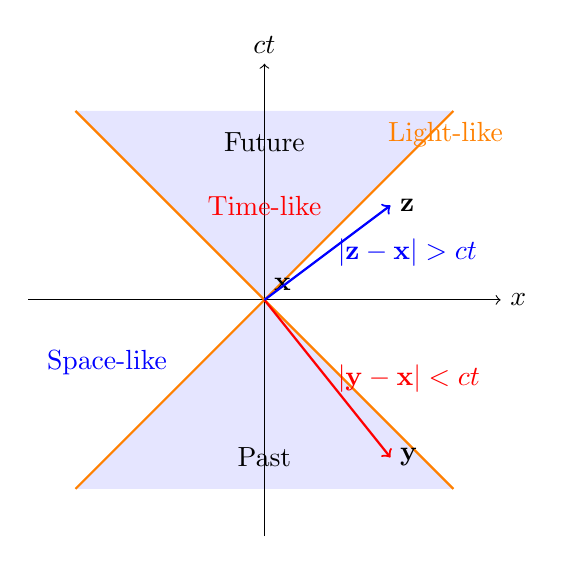
\begin{tikzpicture}[scale=2]

            % Shaded regions (light cone)
            \fill[blue!10] (-1.2,1.2) -- (1.2,1.2) -- (0,0) -- cycle; % future
            \fill[blue!10] (-1.2,-1.2) -- (1.2,-1.2) -- (0,0) -- cycle; % past

            % Axes
            \draw[->] (0,-1.5) -- (0,1.5) node[above] {$ct$};
            \draw[->] (-1.5,0) -- (1.5,0) node[right] {$x$};

            % Light cone lines
            \draw[thick,orange] (-1.2,-1.2) -- (1.2,1.2);
            \draw[thick,orange] (1.2,-1.2) -- (-1.2,1.2);

            % Labels
            \node[above right] at (0.0,0.0) {$\mathbf{x}$};
            \node[right] at (0.8,-1.0) {$\mathbf{y}$};
            \node[right] at (0.8,0.6) {$\mathbf{z}$};
            \node at (0,1.0) {Future};
            \node at (0,-1.0) {Past};
            \node[red] at (0,0.6) {Time-like};
            \node[blue] at (-1.0,-0.4) {Space-like};
            \node[orange] at (1.15,1.05) {Light-like};

            % Vector arrows
            \draw[->,red,thick] (0,0) -- (0.8,-1.0) node[midway,right] {$|\mathbf{y}-\mathbf{x}| < ct$};
            \draw[->,blue, thick] (0,0) -- (0.8,0.6) node[midway,right] {$|\mathbf{z}-\mathbf{x}| > ct$};

        \end{tikzpicture}
    \end{minipage}
    \hfill
    \begin{minipage}{0.45\textwidth}

    \end{minipage}
\end{figure}

\[
    \Delta(x-y) = \frac{1}{4\pi^2} \int \mathrm{d}E_{\mathbf{p}} \sqrt{E_{\mathbf{p}} - m^2} e^{-i E_{\mathbf{p}} t} = \frac{m}{8\pi t} \left(Y_1(mt) + i \frac{J_1}(mt)\right)
\]
where \(Y_1\) is a Besel function of the II kind while \(J_1\) is of the I kind. Now let's take a look at the asymptotic behaviour:
\[
    \begin{aligned}
        J_1(x) & =       \\
        Y_1(x) & = \dots
    \end{aligned}
\]
thus when we take \(t \to \infty \) we get something like \(\sin  - \cos\) so we get
\[
    Y_1(mt) + i {J_1}(mt) \xrightarrow{t \to \infty} i \sqrt{\frac{2}{\pi m t}}e^{-imt},
\]
so that
\[
    \Delta(x-y) = \left[\hat \psi(x),\, \hat \psi(y)\right] \xrightarrow{t \to \infty} \left(e^{-imt} - e^{imt}\right) \neq 0.
\]

The third consideration we have to make is that
\[
    \Delta(x-y) = 0 \quad \forall (x-y)^2<0.
\]
we are computing SPACELIKE separation, in fact outside the light cone
\[
    \begin{aligned}
        \left[\hat \psi(x),\, \hat \psi(y)\right] = \dots pdf \dots
    \end{aligned}
\]
since \(x_0 = y_0 = t\), only the space variables survive in the computation, and the sum of the last two integrals (performing a change of variable from \(\mathbf{p}\) to \(-\mathbf{p}\) on the second integral) we are left with two identical terms subtracted to each other, so we get \(0\). Since this guy is Lorentz invariant, we found this result true for any \((x-y)^2 = - (x-y)^2 < 0\), since the time can be different in \(x\) and \(y\), but we are speaking of spacelike vectors.

We have proven that KG theory mathematically preserve causality (rememner that in RQMPI we looked at how there was a non zero prob of finding a particle propagating at \(v>c\)), let's check this instance phisically: the probability of finding a particle at \(v>c\) should be null.

\section{Klein Gordon Correlators}

Let us consider  particle at a spectime point \(y = (t,\,\mathbf{y})\); how do we describe it in QFT? It is an exhited state of the vacuum \(\ket{0}\), there is some kind of exhitation localized in our quantum field at the point \(y\), like a localized and quantized wave; we recreate it with a creation operator, like \(\hat a_{\mathbf{p}} \ket{0}\), but if we create a particle with definite momentum we could not possibly now its position, so we imagine a linear combination of all possible creation operators with all possible momenta: we apply the \textbf{field operator} on the vacuum
\[
    \hat \psi(y) \ket{0}.
\]
Then let's look at the probability amplitude (with a scalar product) to find it in \(x = (t,\mathbf{x})\):
\[
    D(x-y) = \bra{0} \hat \psi (x) \hat \psi (y) \ket{0}
\]
Note that it is different from RQM, where we computed \(\bra{\mathbf{x}} e^{-i \hat H t} \ket{\mathbf{y}}\) with \(\hat H = \sqrt{\vert \mathbf{p} \vert^2 + m^2}\). Lets compute the amplitude:
\[
    \begin{aligned}
        blablabla \quad pdf \quad blablabla
    \end{aligned}
\]
\(\hat a_{\mathbf{q}}\) acting on the vacuum \(\ket{0}\) is zero, but is the same to \(\hat a^{\dagger}_{\mathbf{q}}\) acting on \(\bra{0}\) (it's just the conjugate of the other); when we see a product of operators, the idea is to use commutators \(\hat a_{\mathbf{p}} \hat a^{\dagger}_{\mathbf{q}} = \left[\hat a_{\mathbf{p}}\, ,\, \hat a^{\dagger}_{\mathbf{q}}\right] + \hat a^{\dagger}_{\mathbf{q}} \hat a_{\mathbf{p}}\); thus we found this amplitude proportional of the \textbf{propagator} (the square modulus of the amplitude gives us the probability of the propagation of the particle from \(\mathbf{y}\) to \(\mathbf{x}\)).

If we evaluate this propagator for propagations outside the light cone (spacelike separation between \(x\) and \(y\), where we consider no time separation and a space separation: \(x-y = (0, \mathbf{r})\), and \(r = \vert \mathbf{r} \vert\)) this should become zero:
\[
    \begin{aligned}
        D(x-y) & =     \\
               & = pdf
    \end{aligned}
\]
if we compute the integral in \(\mathrm{d}(\cos \theta)\) we get to
\[
    D(x-y) = -\frac{i}{2(2\pi)^2 r} \left( \int_0^{\infty} \mathrm{d} \vert \mathbf{p} \vert \dots - \dots \right)
\]
we can compose the integral since we realize it's the same but with different integral domains, so
\[
    D(x-y) = -\frac{i}{2(2\pi)^2 r} \left( \int_{-\infty}^{\infty} \mathrm{d} \vert \mathbf{p} \vert \dots \right)
\]

\begin{figure}[H]
    \centering
    \begin{minipage}{0.45\textwidth}
        \centering
        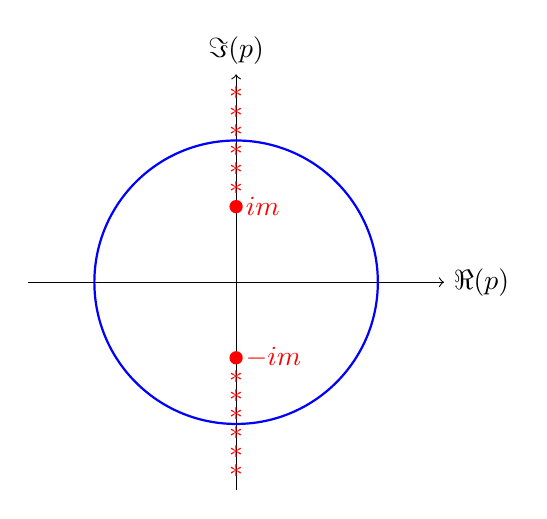
\begin{tikzpicture}[scale=1.2]
            \draw[->] (-2.2,0) -- (2.2,0) node[right] {$\Re(p)$};
            \draw[->] (0,-2.2) -- (0,2.2) node[above] {$\Im(p)$};

            \draw[thick,blue] (0,0) circle (1.5);

            \fill[red] (0.0,0.8) circle (2pt) node[right] {$im$};
            \fill[red] (0.0,-0.8) circle (2pt) node[right] {$-im$};

            \foreach \x in {1.0,1.2,1.4,1.6,1.8,2.0}{
                    \node[red] at (0,\x) {$\ast$};
                    \node[red] at (0,-\x) {$\ast$};
                }
        \end{tikzpicture}
    \end{minipage}
    \hfill
    \begin{minipage}{0.5\textwidth}
        we can now promote module \(\mathbf{p}\) to a complex variable and perform the integral with the couchy theorem; the branch cuts are as shown in figure the same as we have seen in section \ref{sec:RQM_framework}, the ones of a complex square root. We want to get the integral on the real axis, so we compute the path as an integral from \(-L\) to \(L\) on \(\mathbb{R}\) and then we take \(L \to \infty\), then we look at the contributions from the rest of the closed path
    \end{minipage}
\end{figure}

\begin{figure}[H]
    \centering
    \begin{minipage}{0.5\textwidth}
        We have then to compute the integrals on the imaginary axis as \(\vert \mathbf{p} \vert \mathrm{d} \vert \mathbf{p} \vert = -y \mathrm{d} y\) and
        \[
            D(x-y) = \dots = -\frac{1}{2 (2\pi)^2}r 2 \int_{m}^{\infty} \mathrm{d}y \, \frac{y e^{-yr}}{\sqrt{y^{2-m^2}}}.
        \]
        Now this integral is all real without problems, but is it zero?
    \end{minipage}
    \hfill
    \begin{minipage}{0.45\textwidth}
        \centering
        \begin{tikzpicture}[scale=1.1]

            \draw[->] (-2.3,0) -- (2.3,0) node[right] {$\Re(p)$};
            \draw[->] (0,-0.5) -- (0,2.5) node[above] {$\Im(p)$};

            \foreach \y in {1.0,1.2,1.4,1.6,1.8,2.0, 2.2}{
                    \node[red] at (0,\y) {$\ast$};
                }

            \draw[thick,red,<-] (0.2,0.8) arc[start angle=0,end angle=360,radius=0.2] node[right] {$C_{\epsilon}$};

            \draw[thick,->,green] (-2.2,0) -- (-1,0);
            \draw[thick,->,green] (-1,0) -- (1,0) node[below] {$C_L$};
            \draw[thick,green] (1,0) -- (2.2,0);

            \draw[thick,orange,
                postaction={decorate},
                decoration={markings, mark=at position 0.5 with {\arrow{<}}}
            ] (-2.2,0) arc[start angle=180,end angle=90,radius=2.2] node[above right] {$C_1$};

            \draw[thick,orange,
                postaction={decorate},
                decoration={markings, mark=at position 0.5 with {\arrow{>}}}
            ] (2.2,0) arc[start angle=0,end angle=90,radius=2.2] node[above left] {$C_4$};

            \draw[thick,->,blue] (0.1,2.2) -- (0.1,1.0) node[above right] {$C_2$};
            \draw[thick,<-,blue] (-0.1,2.2) -- (-0.1,1.0) node[above left] {$C_3$};

            \fill[red] (0,0.8) circle (2pt) node[right] {};
            \fill[black] (-2.2,0) circle (2pt) node[below] {$-L$};
            \fill[black] (2.2,0) circle (2pt) node[below] {$L$};

        \end{tikzpicture}
    \end{minipage}
\end{figure}

No, the exat solution is given in terms of modified bessel functions, and in the limit for \(r \sim \infty\) then \(D(x-y) \sim e^{-mr} \neq 0\) even if \(r\) is really big. but we can arrive at the same solution with approximated considerations.
This seems similar to what we obtained in RQM, but it is not: indeed if we consider the previous result
\[
    \Delta(x-y) = \left[\hat \psi(x),\, \hat \psi(y)\right] = 0
\]
for spacelike separations, so we can write
\[
    \begin{aligned}
        \Delta(x-y) & = \bra{0}\Delta(x-y)\ket{0} = \bra{0} \left[\hat \psi(x),\, \hat \psi(y)\right] \ket{0}                  \\
                    & = \bra{0} \hat \psi(x) \hat \psi(y)\ket{0} - \bra{0} \hat \psi(y) \hat \psi(x)\ket{0} = D(x-y) - D(y-x);
    \end{aligned}
\]
Note that KG theory cannot distinguish particles from antiparticles, since it does not account for charge degrees of freedom, so we can interpret this result as the probability amplitude for a particle to go from y to x minus the probability of the antiparticle going from x to y, which is an interpratation of antiparticles going backward in time to preserve the causality outside the light cone.

If we want a state in which we have a particle in the past and then in the future, we can also read this as a particle in the past, then the creation of a couple of part antipart in the future, the new particle stays in the future while the antiparticle travels backwards in time to annihilate with the initial particel. We were compiting just one half of the amplitude. All this comes from intrepretation of the athematical results of our equations. We are looking at one individual phenomenon made up by two distinct contributions.

\[
    DRAWS \, FROM \, PDF
\]
We are summing diagrams where before \(y\) and after \(x\) we have the same phenomenon, but between \(x\) and \(y\) we have in a case the particle propagating faster than light, in the other the produced antiparticle traveling backward in time faster than light only to annihilate with the other old particle in \(y\). This physical intuistion is mostly due to Feynman and his diagrams.

This kind of phenomena are called \textit{virtual phenomena}, since they cannot be measured observed, but mathematic tells us that this happens and saves our theory; even in Feynman diagrams, the virtual particle does not respect an equation of motion, there is its existence for a really brief moment, and due to uncertainty in energy etc we can justify its existence and our computing methods and interpretations.


\subsection{Green Functions}

\subsection{Feynman Propagator}